\chapter{Introduction}
\label{chap:introduction}

%Through language, humans are able to change the world by requesting that others do things, by asking for new information, and by providing new information themselves. It is hard to imagine what the human species would be without these fundamental linguistic capacities.
We can use language to do a great many things, such as warning, arguing, guessing, pleading, naming or declaring. But from the point of view of linguistics, three particular kinds of speech acts appear to stick out.
These are the broad classes of assertions, questions and commands (or requests). They are special because
languages tend to have dedicated three clause types to the performance of these three kinds of speech acts (\citealt{sz1985speechact, konig2007, aikhenvald2016, portner2018}, see \cite{konig2020} for a recent review). Declaratives are typically used for assertions (\ref{ex:intro:intro:dec}) and (\ref{ex:intro:man:dec}), interrogatives for questions (\ref{ex:intro:intro:int}) and (\ref{ex:intro:man:int}), and imperatives for commands (\ref{ex:intro:intro:imp}) and (\ref{ex:intro:man:imp}):

\bex{ex:intro:intro}
English clause types:
\bxl \label{ex:intro:intro:dec}
That's Elmo. \hfill Declarative, Assertion
\ex\label{ex:intro:intro:int} Is that Elmo? \hfill Interrogative, Question
\ex\label{ex:intro:intro:imp} Find Elmo! \hfill Imperative, Request
\exl
\eex

\bex{ex:intro:man}
Mandarin clause types:
\bxl \label{ex:intro:man:dec}
\gll Zhe shi Elmo.\\
This is Elmo\\
\trans ``This is Elmo.'' \hfill Declarative, Assertion
\ex \label{ex:intro:man:int}
\gll Zhe shi Elmo \tbf{ma}?\\
This is Elmo \Sfp\\
\trans ``Is that Elmo?'' \hfill Interrogative
\ex \label{ex:intro:man:imp}
\gll Zhizhi Elmo!\\
Point Elmo\\
\trans ``Point at Elmo!'' \hfill Imperative
\exl
\eex

While the functions stay constant, the form varies from language to language. As the above examples in English and Mandarin show,  both English and Mandarin have declaratives, interrogatives, and imperatives to perform the functions of asserting, questioning, and commanding, respectively. But the form of each clause type in these two languages differ. For example, if we compare the interrogative clauses in the two languages with the declarative clauses, we can see that the English interrogative clause has a different word order than the English declarative clause, with the subject and the auxiliary switching places in the interrogative clause. In Mandarin, the difference arises at the edge of the sentence, as the interrogative clause has an additional sentence final particle \tit{ma} at the end of the sentence. In Mandarin, one can also use A-not-A constructions for polar interrogatives:

\bex{ex:intro:anota}
\gll Zhe \tbf{shi-bu-shi} Elmo?\\
This be-\Neg-be Elmo\\
``Is this Elmo?'' \hfill A-not-A Interrogative
\eex

The canonical function of such sentences is to perform a questioning speech act, just like its English counterpart (\ref{ex:intro:intro:int}), but interrogativity in this example is marked by the presence of the disjunctive negative structure (i.e. \tit{shi-bu-shi}). 

Besides using relative word order of constituents (English), particles (Mandarin \tit{ma}), or disjunctive negative structures (Mandarin A-not-A), we also find languages like West Greenlandic that differentiate the two clause types by verb inflection:

\bex{ex:intro:gl}
West Greenlandic
\bxl
\label{ex:intro:gl:dec}
\gll neri- vutit\\
eat- \Ind.\Ssg.\Pst{}\\
``You ate.'' \hfill Declarative
\ex \label{ex:intro:gl:int}
\gll neri- vit\\
eat- \Int.\Ssg.\Pst{}\\
``Did you eat?'' \hfill Interrogative
\exl
\hspace*{\fill} \cite[18, ex (50)]{konig2007}
\eex

As (\ref{ex:intro:gl}) shows, West Greenlandic uses the suffix \tit{vutit} for declaratives and \tit{vit} for interrogatives.

\revise{Morpho-syntactic features are not the only way to differentiate clauses in languages. In languages like Italian and Portuguese, declaratives and interrogatives share the same morpho-syntactic features and only differ in intonation, as shown in Figure~\ref{fig:intro:PB}:}
\begin{figure}[H]
    \centering
    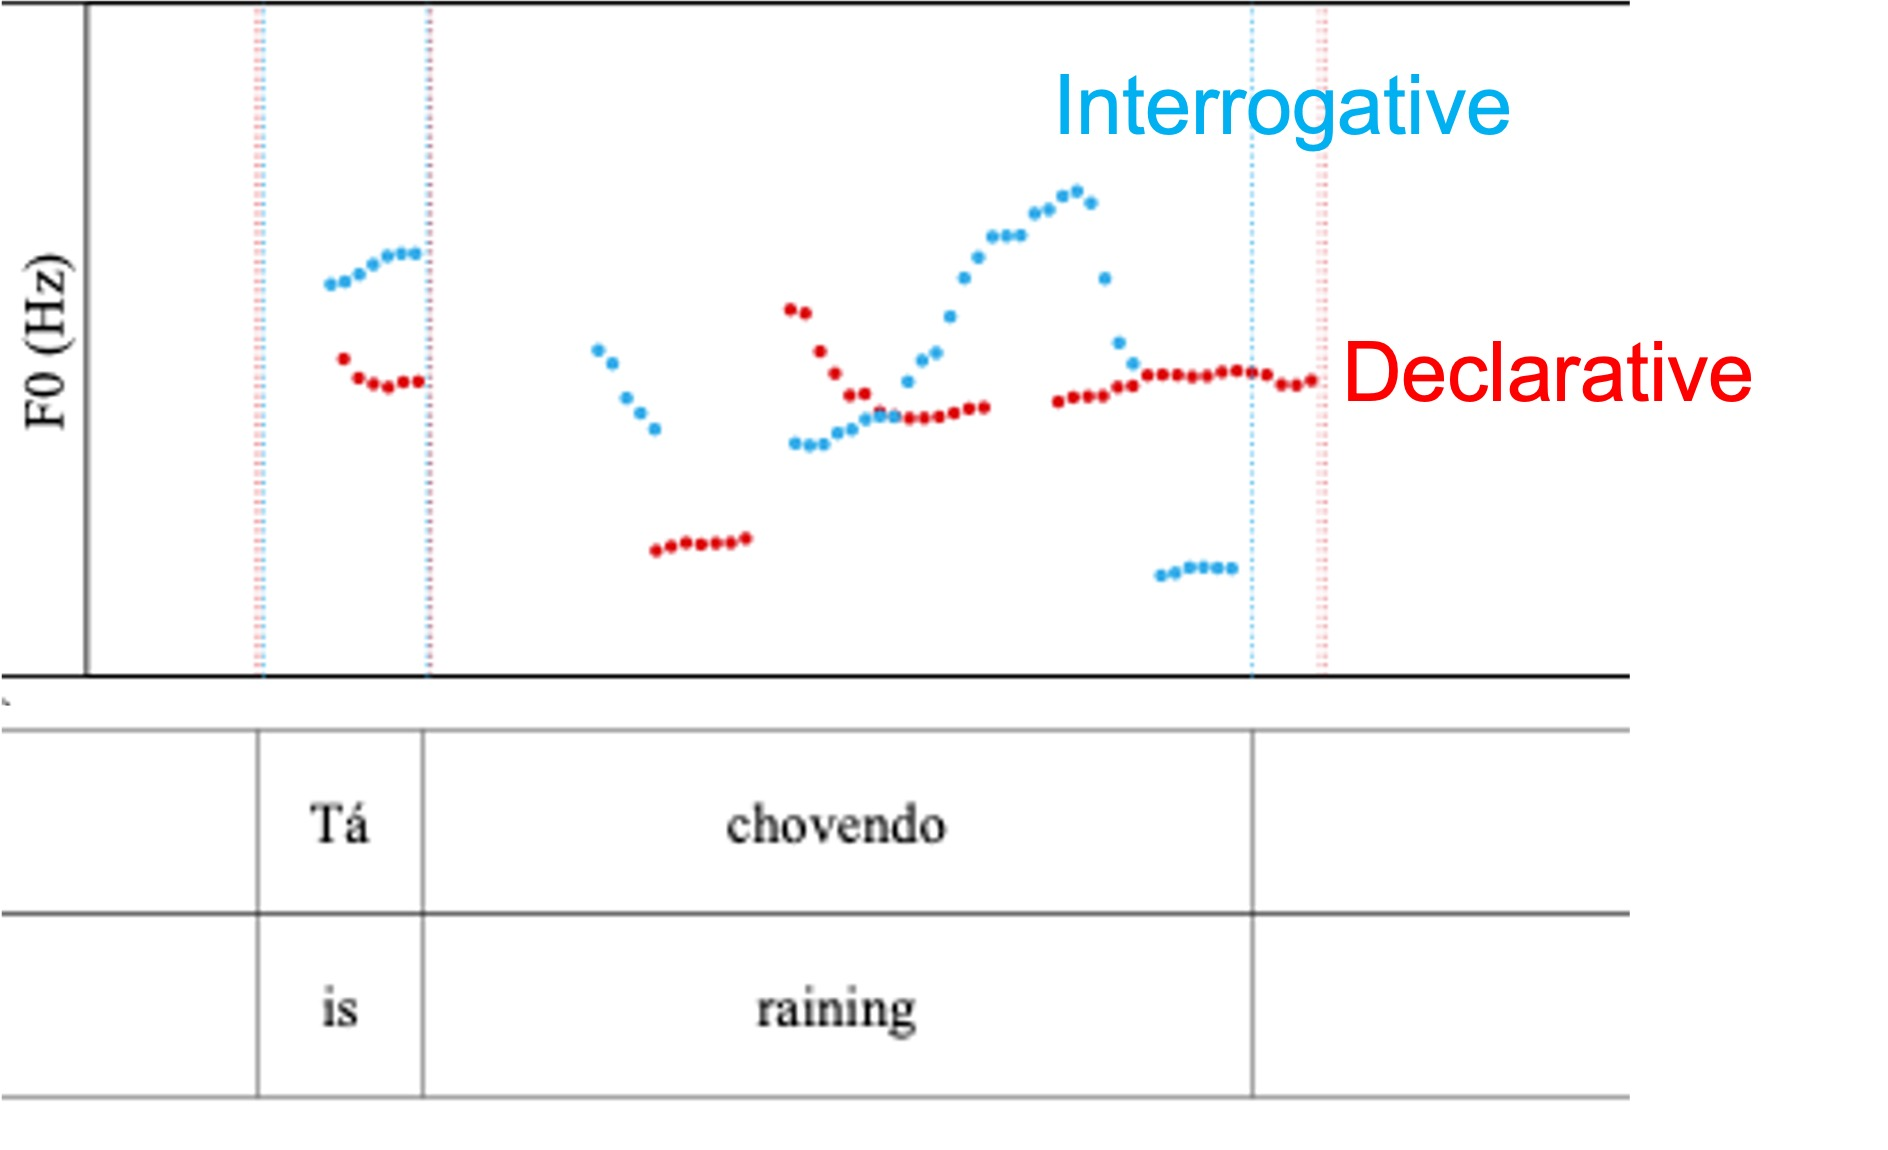
\includegraphics[width=0.7\textwidth]{figures/PB.jpg}
    \caption{F0 of declarative and interrogative sentences in Brazilian Portuguese (p.c. J\'essica Mendes)}
    \label{fig:intro:PB}
\end{figure}

\revise{In Portuguese, interrogative and declarative clauses could be string-identical, and the only difference lies in their pitch contour (see \cite{truckenbrodt2009prosody} for discussion on a detailed discussion of the role that intonation played in differentiating clause types and speech acts in Portuguese). }

For \twh-interrogatives, languages differ in whether the \twh-phrase is fronted to the beginning of a clause,  like English (\ref{ex:intro:engwh}), or stays in situ, like the Mandarin sentence in (\ref{ex:intro:manwh}):

\bex{ex:intro:engwh}
\tbf{What} did Elmo eat?
\eex

\bex{ex:intro:manwh}
\gll Elmo chi-le \tbf{shenme}?\\
Elmo eat-\Asp{} what\\
``What did Elmo eat?''
\eex

Despite all these cross-linguistic differences in how the clause type information is encoded in the surface form, we can still see that in each language, we find these three major clause types (\diis{}) that are canonically associated with the same three major speech acts (\aqrs{}). 

\revise{People refer to this mapping between form and meaning as the \tit{sentential force} or \tit{Mood}. what in fact needs to be learned in our situation, is a semantic category underlying the clause type category and speech act category, namely \tit{mood} or \tit{sentence force}. This category is systematically related to (a) syntactic distribution (i.e. the distribution of formal features that we are currently assuming to be associated with clause type features) and (b) pragmatic functions (speech acts). Observations of only the formal distribution or only the pragmatic function had the potential to mislead, and so the learners need both to mutually constrain each other. }

Of course, matters are not quite so simple. While each of the three major clause types bears a canonical association with one of the major speech acts, this mapping is not inviolable. One can use a sentence with a particular clause type to perform a speech act other than the canonically associated one. For example, when we use the sentence \tit{Can you pass the salt?} at the dinner table, then, even though the sentence is clearly an interrogative in English with subject-auxiliary inversion, the speech act performed by the speaker is best characterized as a requesting act. The same is true in Mandarin:

\bex{ex:intro:manmis}
\gll Keyi bang wo diyixia zhijin \tbf{ma}?\\
Can help me pass napkin \Sfp{}\\
``Can you pass me the napkin?''
\eex

Sentences with the particle \tit{ma}, as discussed above, are interrogatives in Mandarin. But just like its English counterpart, when you utter (\ref{ex:intro:manmis}) to someone sitting next to the napkin box, you are making a request rather than asking a question. 

Thus, although languages tend to have dedicated clause types that are typically associated with particular speech acts, these clause types can be used for other speech acts. 

As adults, we effortlessly understand this canonical association between clause types and speech acts -- and when it is violated. When we hear someone utters ``Is it raining?'' we assume that they are asking a question, and when we hear someone says ``It's raining!'' we assume that they are making an assertion.  But for a child whose grammar is still developing, this might not be trivial, as they have to figure out the makeup of the \diis{} in their language and associate them with their canonical speech acts.   %How do they figure out speech act, if they can’t rely on clause types, and conversely, how can they figure out clause types, if they need clause types to figure out speech acts? how does a child figure out the clause types in their language, and link them to their canonical functions?

Remarkably, children seem to have figured this out from a young age. By 18 months, they seem to be able differentiate interrogatives from declaratives, and understand that people use interrogatives to ask questions, all while their grammar and understanding of the world are still in development (\cite{geffenmintz2011,geffenmintz2015wordorder,casillas2017turn,perkins2019,marshmallowqueen} among others). In this dissertation, I examine how children can figure out clause typing and how they learn to associate the three major clause types with the three major speech acts. %The existence of three clause types and the mapping between clause types and speech acts seem to be robust across languages, but ? Specifically, children first need to sort the sentences of their language into three categories that correspond to the three clause types (the ``clustering problem''). Second, they need to figure out which category is canonically associated with which speech act speech act (the ``labeling problem'').

%A child learning English who has sorted \emph{Is it raining?}\ and \emph{It is raining!}\ in the same category has not identified the English clause types and thus has not solved the clustering problem. A child who has learned that \emph{Is it raining?}\ and \emph{It is raining!}\ go into different categories, and has only sorted interrogatives with \emph{Is it raining?}\ and only declaratives with \emph{It is raining!}, has solved the clustering problem -- but if it labelled the cluster containing \emph{Is it raining?}\ as the cluster of sentences typically used to perform assertions, then it has not solved the labelling problem. 

In the rest of this chapter, I first explain in detail the two learning problems related to clause type categories (Section~\ref{sec:intro:cl:problem}). In Section \ref{sec:intro:cl:prag}, I explore the relevance of information about speech acts to the task of learning clause types. Then, in Section~\ref{sec:intro:hypo}, I detail my plan for probing the question of how children might figure out the right clause types, and in Section \ref{sec:intro:sp}, I address the remaining issue of learning speech acts. Finally, in Section~\ref{sec:intro:roadmap} I summarize the different aspects of the problem and lay out the roadmap of this dissertation. 

\section{Learning clause types}
\label{sec:intro:cl}
\subsection{The clustering and labeling problem}
\label{sec:intro:cl:problem}

As we have seen, languages tend to have three clause types.  Given the near-universality of these main clause types, it may be reasonable to assume  that children expect that their language is likely to have three main clause types. But even if we assume that the knowledge of clause type categories is innate, learners still face two main problems.

First, input sentences do not wear their clause type categories on their sleeves. Rather, learners need to identify the specific signals in the surface form of the sentences in their language that are associated with the three clause types. That is, they need to identify the right formal properties of sentences that allow them to categorize a sentence with all other sentences of the same clause type. This is the \tbf{clustering problem}.
To use English as an example, English-acquiring children have to figure out that (\ref{ex:intro:cluster-base}) shares its clause type with (\ref{ex:intro:cluster:dec}), even though they have different lexical items, because the subjects in both follow the auxiliaries; but also that (\ref{ex:intro:cluster-base}) has a different clause type than (\ref{ex:intro:cluster:dec}) even though both share the same lexical items, because the subject in the latter precedes the auxiliary. The learner needs to recognize that subject-auxiliary inversion is a formal feature that is relevant for clause typing.

\bex{ex:intro:cluster-base}
Do you want a cookie?
\eex
\bex{ex:intro:cluster}
\bxl\label{ex:intro:cluster:int}
Is that Elmo?
\ex\label{ex:intro:cluster:dec}
That’s Elmo!
\exl
\eex

\begin{comment}
Meanwhile, Mandarin-acquiring children have to figure out that \ref{ex:intro:man:cluster-base}

\bex{ex:intro:man:cluster}
\eex
\bex{ex:intro:man:cluster-base}
\bxl
\gll Zhe shi Elmo.\\
This is Elmo\\
\trans ``This is Elmo." \hfill Declarative
\ex 
\gll Zhe shi Elmo \tbf{ma}?\\
This is Elmo \Sfp\\
\trans ``Is that Elmo?'' \hfill Interrogative
\exl
\eex
\end{comment}

Second, after identifying the clusters, learners need to determine the canonical function of each cluster in the system. That is, after clustering sentences into three categories, children still need to learn which one of these clusters is the interrogatives (typically used to perform questions), which is the declaratives (typically used to perform assertions), and which is the imperatives (typically used to perform commands). This is the \tbf{labeling problem}. %As adults, when we hear someone say ``Is it raining?'' we assume that they are asking a question, and when we hear someone says ``It's raining!'' we assume that they are making an assertion.  But for a child whose grammar is still developing, this might not be trivial, as they have to figure out the makeup of the \diis{} in their language and associate them to their canonical speech acts.  


Solving these two problems is neither trivial nor straightforward. For the clustering problem, each clause type cateogry is related to a variety of surface forms, none of which is obligatorily present and many of which can occur in sentences with a different clause-type category. For example, as we have discussed, in English, the hallmark of interrogativity is subject-auxiliary inversion, which can be seen in polar interrogatives (\ref{ex:intro:cluster:int}) and \twh-interrogatives (\ref{ex:intro:engwh2}) below. However, this association of word order and interrogativity has many exceptions. Subject \twh-interrogatives like (\ref{ex:intro:engwhsubj}) do not have this formal feature.


\bex{ex:intro:engwh2}
Who \tit{can} \tbf{Sue} hug? \hfill Object \twh{}, Subject-Auxiliary Inversion
\eex
\bex{ex:intro:engwhsubj}
\tbf{Who} \tit{can} hug Ann? \hfill Subject \twh{}, no Subject-Auxiliary Inversion
\eex

\begin{comment}
Similarly, in embedded clauses, we also do not see subject-auxiliary inversion: 
\bex{ex:intro:eng-embed}
Mary wonders $[_{\Int}$ whether \tbf{Ann} \tit{can} hug Elmo].
\eex

As shown in (\ref{ex:intro:eng-embed}), the auxiliary \tit{can} and subject \tit{Ann} of the embedded interrogative have the same word order as a matrix declarative sentence.
\end{comment} 

Conversely, some morpho-syntactic properties typically associated with interrogative clauses could also appear in other settings. For example, in English, some declaratives exhibit subject-auxiliary inversion: 

\bex{bg-syn:dec}
\bxl\label{bg-syn:decreg}
Mary would never eat tripe in her life. 
\ex\label{bg-syn:decneg} Never in her life would Mary eat tripe.
\exl
\eex

In English, fronting the negator \tit{never} can cause the raising of an auxiliary, giving the sentence an appearance of subject-auxiliary inversion, but the clause type category is not interrogative. %Both (\ref{bg-syn:decreg}) and (\ref{bg-syn:decneg}) are declaratives, but when the negator \tit{never} is fronted as in (\ref{bg-syn:decneg}), the auxiliary precedes the subject.

Therefore, learners need to infer the right clause type category of sentences they hear in the input, but they might not see the crucial surface morpho-syntactic features for clause typing, or the surface features that they do see misalign with the actual clause type category of the sentence. A particular formal feature can, in principle, occur in sentences having different clause types, and sentences having a particular clause type can have different formal features. Thus, even a learner who is able to, for example, recognize subject-auxiliary inversion might have difficulty to recognize its role for determining interrogativity.

But this many-to-many mapping problem is not the only challenge for learners to face when solving the clustering problem. Learners also have to deal with cases where the relevant morpho-syntactic features are masked, for instance, by other syntactic operations. For example, left-edge-ellipsis is such an operation (\cite{zwickypullum1983leftedge}):

\bex{ex:intro:lee}
Want to go out
\eex

The string in (\ref{ex:intro:lee}) could result from eliding the subject pronoun from a declarative clause like (\ref{ex:intro:lee-unpack}a), or result from eliding the subject and the auxiliary from a polar interrogative like (\ref{ex:intro:lee-unpack}b). But the surface form of (\ref{ex:intro:lee}) itself does not have enough information to help us identify its clause type feature.\footnote{Note that the intonation would not help in this case either, because both (\ref{ex:intro:lee-unpack}a) and (\ref{ex:intro:lee-unpack}b) are likely to have a final rising contour L* H-H\% (\cite{gunlogson2008, jeong2018, goodhue2021rd}). } 

\bex{ex:intro:lee-unpack}
\bxl
You want to go out?
\ex Do you want to go out?
\exl
\eex

%These problems are not specific to English. In fact, Mandarin provides lots of cases where the formal features for clause typing are misaligned or absent. %This problem is especially prominent with \twh-interrogatives/

\begin{comment}
In Mandarin, the presence of \twh-phrases and question particles are the two hallmarks of Mandarin interrogatives. But in \twh-interrogatives, the question particle \tit{ne} is optional, and \twh-phrases do not move to sentence initial position. As a result, in some cases like (\ref{ex:intro:man-ne}b), the only difference between the interrogative sentence and its declarative counterpart is the presence of \twh-phrase:

\bex{ex:intro:man-ne}
\bxl
\gll Elmo chi-le dian \tbf{shenme} \tbf{ne}?\\
Elmo eat-\Asp{} \Cl{} what \Sfp{}\\
``What did Elmo eat?''
\ex \gll Elmo chi-le dian \tbf{shenme}?\\
Elmo eat-\Asp{} \Cl{} what\\
``What did Elmo eat?''
\exl
\eex 

\bex{ex:intro:man-np}
\gll Elmo chi-le dian binggan\\
Elmo eat-\Asp{} \Cl{} cookie\\
``Elmo ate some cookies.''
\eex

However, declarative sentences could also have \twh-phrases, where these phrases are interpreted as indefinites like English \tit{any/a} (\cite{huang1982, cheng1991,LMYY2021}). %As a result, a string like (\ref{ex:intro:m-whamb}) could be either an interrogative (interpretation a) or a declarative (interpretation b). 


\bex{ex:intro:m-whamb}
\gll Xiaoxiao mei 	chi 	\tun{shenme} dongxi\\ 
Xiaoxiao \Neg{} 	eat	what	things\\
a.	``What didn’t Xiaoxiao eat?''	\hfill Interrogative \twh\\
b.	``Xiaoxiao didn’t eat anything.''		\hfill Indefinite \twh
\eex

In (\ref{ex:intro:m-whamb}), the interrogative version of the string 
\end{comment}

The problem is even more prominent in languages like Mandarin where the morphological cues are scarce. For example, the absence of subject is a feature of imperatives in Mandarin, same as English, but since Mandarin is a pro-drop language, subjects are frequently elided, regardless of the clause type. As a result, it is likely that a learner observes more subject-less non-imperative sentences than imperative sentences.  



Thus, even if we assume that the learners come with the expectation that their language is likely to have three clause types, they still have to figure out the right clustering of the clauses (the clustering problem), and label the clusters with the canonical functions of the clauses (the labeling problem). They might face many challenges when solving the two problems, as the formal features for one clause type category might not show up in the surface string, or might appear in sentences of another category. Could children learn clause typing from surface features alone? 

As already mentioned, cross-linguistically, we see a robust association of the three major clause types with the three major speech acts. Might this association itself be a useful source of information to the learner?

\subsection{The usefulness of speech act information}
\label{sec:intro:cl:prag}

At the beginning of this chapter, we saw that cross-linguistically, declaratives are canonically mapped to assertions, interrogatives to questions, and imperatives to commands. Could exploiting this mapping potentially help the learner? Let's consider this hypothesis and evaluate how pragmatics might help a learner to solve the clustering and labeling problems.

Clearly, having access to some speech act information is necessary to solve the labeling problem: to understand that a particular clause type is declarative (i.e.\ typically used for asserting) and another is an interrogative (i.e.\ typically used for questioning), it is not just useful but indeed \emph{necessary} for a learner to be able to recognize some speech act information. Absent such information, there would be no way to associate a particular cluster with a particular speech act type.

As for the clustering problem, surface formal features alone may suffice to allow a learner to cluster sentences into three distinct formal categories. However, as we discussed in the last section, the formal features for one clause type category might not show up in the surface string, or might appear in sentences of another category. The question then is, is the surface formal features of the sentences that the learners observe in their input sufficient for identifying the right three clause types? If not, what information might bridge this gap between learners' input and the abstract clause type categories they need to acquire? That is, what information might help learners bootstrap into the abstract clause type categories (cf. \cite{pinker1984, gleitman1990, hacquardlidz2018})? 

The obvious candidate for a source of information that goes beyond formal features is again information about the speech act being performed. We have seen that cross-linguistically, the three clause type categories are systematically related to three speech acts. If learners know that there are three clause types that are associated with three speech acts and are able to observe that sentences with subject-auxiliary inversion are often or predominantly appear in sentences that are used for questioning, this might help them to recognize the relevance of subject-auxiliary inversion for clause typing. The same can be said about other formal features. Thus, despite our observation that the mapping between the three major clause types and the three major speech acts is many-to-many, learners could take advantage of pragmatic information related to speech act type to fill in the gaps left by surface formal features in the input. 

\subsection{The problem with speech act information}
The mapping between clause types and speech acts could also hurt children's chances of learning clause types, again because this mapping too is many-to-many. In some contexts, it is possible that the conventionalized speech act associated with a clause type is not the actual speech act performed by uttering it. \tbf{Indirect speech acts} are these mismatching cases where the primary, ``non-literal'' speech act of an utterance is different from the conventionalized, ``literal'' speech act of a sentence associated with its clause type (\citealt{searle1975tax, searle1976class, bachharnish1979, searlevanderveken1985, portner2004, starr2014, portner2018, murraystarr2020} a.o.). As we have discussed briefly at the beginning of the chapter,  when you utter \tit{Can you pass the salt?} at the dinner table, it is likely that you intent this utterance to be taken as a request. As an interrogative clause with subject-auxiliary inversion, its conventionalized (and ``literal'') act is questioning, but the primary act performed is requesting. As a result, some speech act categories can be expressed by more than one clause types, and vice versa. For example, interrogatives can express assertions, questions, requests/commands. You can use the interrogative sentence in (\ref{eng-cl:int-asst}) to assert that the Linguistics Department is on the UPPER floor as a correction to your friend who thinks that the department is on the third floor; or you can use the interrogative sentence in (\ref{eng-cl:int-req}) to request your friend to pass the salt to you.

\bex{eng-cl:int-all}
Speech acts expressed by interrogatives 
\bxl Is it snowing? \hfill Question
\ex \label{eng-cl:int-asst} Isn't our department on the UPPER floor of Marie Mount Hall? \hspace*{\fill} Assertion
\ex\label{eng-cl:int-req} Can you pass the salt? \hfill Request
\exl
\eex

Conversely, questions can be expressed by \diis{}. You can utter any of the sentences in (\ref{eng-cl:q-all}) to perform a questioning act. 


\bex{eng-cl:q-all}
Clause types expressing questions
\bxl
Is it raining? \hfill Interrogative
\ex I wonder if it's raining. \hfill Declarative
\ex Tell me if it's raining! \hfill Imperative
\exl
\eex

If such mismatching cases are prevalent in children's input, the speech act information might not be helpful for children to figure out clause types. Just like the problem with formal features was that they might not appear to be uniquely associated with a single clause type, the problem with speech act types is that they are also not uniquely associated with a single clause type.


\subsection{Learning clause types: Interim summary}
\label{sec:intro:hypo}

To summarize our discussion so far, we have seen that languages tend to have three clause types dedicated to three speech acts, and as we will see in the next chapter, by 18 months old, children seem to be able to differentiate these clause types and associate them with their canonical speech act. To gain this ability, they need to identify the right categories of clauses (the clustering problem) and figure out what speech act they are canonically used for (the labeling problem). To solve the labeling problem, some speech act information must be available, but if there are too many mismatching cases between speech acts and clause types, this information might not be useful after all. To solve the clustering problem, children need to pay attention to the surface morpho-syntactic features of each sentence in their input. But in the input, the surface features might be absent or misleading. Again, it seems plausible that speech act information can help, but this information too is potentially misleading.

This dissertation therefore investigates these questions: first, are the surface formal features of the sentences in the input sufficient for children to figure out the clustering of clause types? Second, if not, is speech act information helpful or hurtful? 

I compare two learners, a \distlearner{} (\dlearnerabbr{}), and a \praglearner{} (\plearnerabbr{}). Both learners use the surface morpho-syntactic features of the input sentences to attempt to cluster sentences into three categories, i.e.\ to learn the clause type categories. But the \plearnerabbr{} additionally has access to information about which speech act is performed by a sentence. In Chapter~\ref{chap:eng-cl}, I simulate these two learners with Bayesian clustering models on English data. By comparing the performance of the two models, I show that morpho-syntactic features alone is not sufficient to learn the three clause types, but adding information about speech act type suffices to learn the clause types, even if the speech act information is noisy. I conclude that speech act information is helpful, indeed crucial, to solve the clustering problem.

In Chapter~\ref{chap:man-cl}, I test the models' performance for learning Mandarin clause typing, where the learners need to use a different set of surface features for clause typing. Moreover, due to its impoverished morphological system, the surface formal features for clause typing might be even more likely to be absent or misaligned. The results from the two models suggest that the surface formal features in Mandarin are even less informative for clause typing than in English; without speech act information, the learner might not be able to identify any clause types.  

This insufficiency of syntax leads us to the following \tbf{\subhypos{}}:
%\begin{comment}
\begin{quote}
Infants use the speech act information, in addition to observations of morpho-syntactic features in the surface form of sentences, to cluster and label input sentences into the three major clause types.
\end{quote}
%\end{comments}


This hypothesis states that to compensate for the insufficiency of surface formal features, children need to use the speech act information to bootstrap into clause type categories.



\section{Learning speech act categories}
\label{sec:intro:sp}

At first glance, it appears that for the \subhypos{} to work, we have to assume that in order to have figured out the clause type categories, children need to have figured out how to obtain speech act information. But this might catch us in a chicken-and-egg problem.

While some evidence suggests that 18-month-olds can infer speech acts, especially questions (\cite{casillas2017turn, marshmallowqueen}), their inferences might not be perfect, so they might misidentify some or many speech acts. That is, children might have only limited access to speech act information. Moreover, there is the problem of how children can infer speech act categories in the first place -- and it is undeniable that the clause type information is useful for solving this problem. As adults, the primary way we identify the speech act performed by a given sentence is through its clause type. But this is precisely the problem that the child is trying to solve (i.e. identifying the clause type). If children need speech act information to learn to identify clause type categories, but they also need clause type information to identify speech act categories, it seems that we have a chicken-and-egg problem. 

This way of putting the problem makes it seem like children have to either first learn to recognize speech acts and, having done this, move on to learn to recognize clause types, or first learn to recognize clause types and, having done this, move on to learning to recognize speech acts. But it is not a given that 
that learning clause types and learning speech acts happen sequentially like that. Quite the opposite, it is likely that children learn to identify speech act and clause type in tandem and mutually informative ways: children learn to identify clause types by tracking formal regularities in conjunction with their growing
knowledge of speech act and its associated social-pragmatic cues; simultaneously, they learn
to identify speech acts by tracking socio-pragmatic cues in conjunction with their growing
understanding of the formal features of various clause types.


To get one step closer from our \subhypos{} to the \tbf{\hypos{}}, I first ask how much speech act information children need to identify clause types. If children do not need \emph{perfect} speech act information to figure out clause types, then we do not need to assume that by the time children are learning to figure out clause types, they have already figured out speech acts. %half of the \hypos{}, namely that children learn to identify clause types by tracking formal regularities in conjunction with their growing knowledge of speech act, could be feasible. 

In Chapter~\ref{sec:engcl:model:noisy} and Chapter~\ref{sec:mancl:model:results:noisy}, I simulate the learning of clause type with various degrees of noise in the speech act information, so that we can see how much pragmatics a learner needs to succeed at the clustering problem. The results suggest that even if learners only have limited access to pragmatics, they could still benefit from this source of information. This allows us to abandon this misleading way of formulating the problem, that the learning of clause types has to happen after the learning of speech acts.

I then %address the second problem
ask what kind of non-clause type cues for speech act information are present in the input. Even if children must rely on clause type information to figure out the speech acts, they could have access to additional information that is unrelated to clause typing, but informative for recognizing speech act type. For example, in conversations, we use questions to elicit responses and information, which leads to behaviors like pausing after questions, or looking directly at our interlocutor, to nudge them to answer our questions. 
This in turn means that we can expect different kinds of behavior to be correlated with each speech act. Thus, for instance, armed with an innate category for questions (e.g. \cite{carruthers2018q}\footnote{\textcite{carruthers2018q} argues that what is innate is the questioning \tit{attitude} (the desire to know to be more precise), which for him is what gives us the act of questioning.  }), and a theory of what questions do in conversations, the child can expect certain kinds of nonlinguistic behavior to be somewhat correlated with the act of asking a question. 

Some candidates for cues that could potentially differentiate questions from other speech acts are prosody, pauses, and direct eye gaze. Cross-linguistically, pitch rises tend to signal questions and pitch falls signal assertions; and some argue that this universality reflects the innate knowledge that high rising pitch connects to the speech act of questioning (\cite{ohala1984,gussenhovenchen2000,gussenhoven2002} among others). If children are armed with this knowledge that questions are associated with rising contours, they might expect rising contours to be correlated with the act of asking a question. If the input is such that more questions are uttered with rising contour than assertions, then this could be helpful for the child to figure out what utterances are  questions in their input. But just as not all interrogatives have subject-auxiliary inversion and not subject-aux inversion are interrogatives, not all questions have final rises (\cite{gussenhoven2000fallq, hedberg2004wh,ladd2008intonational}), and not all final rises are questions (e.g. \cite{gordon1999prosody,ladd1981, ward1985rfr,goodhue2016prosody}). In English, \twh-questions are usually produced with final fall (\cite{hedberg2004wh,ladd2008intonational}), and the rise-fall-rise contour could be associated with assertions (\cite{ladd1981, ward1985rfr,goodhue2016prosody}). Nevertheless, it is still possible that more questions than assertions are produced with rises in the input, which could still be informative for the child. We therefore need to verify empirically whether prosodic information is potentially informative.

The canonical function of questions is to solicit responses or seek information (\citealt{searle1975tax,levinson1983,stivers2010}, see \citealt{krifka2011q} for a recent overview). When we use questions, it is likely that we pause after questions, or look directly at our interlocutor, as a way to signal to them that they need to take over the conversational turn. If children have prior knowledge that certain speech act is used for response-elicitation, and if they know that pauses and direct eye gaze are how humans signal their expectations of a reciprocation of communication, then they may expect questions to be correlated to some degree with longer pauses and direct eye gaze. Again, this is something that needs to be checked empirically.

If children have such expectations, would they find anything in the input? In Chapter~\ref{chap:eng-sp}, 
I conduct a corpus study examine the prosody of English-speaking parents' utterances (Section~\ref{sec:engsp:results:prosody}), length of pause after utterances (Section~\ref{sec:engsp:results:pause}), and proportion of eye gaze around the time of an utterance (Section~\ref{sec:engsp:results:gaze}). 


I find that parents do not use final rises more often with questions, but polar interrogatives have more final rises than other types of speech acts and clause types, including \twh-interrogatives and declaratives. As for the two behavioral cues, parents tend to pause longer after questions, and attend the child more when asking questions. To the extent that they are weakly correlated with the questioning act, it is in principle plausible that (a) a child could use these features, in addition to their growing knowledge of clause types to infer the speech act category of an utterance; and (b) this little bit of information about speech act could then be used to provide the noisy pragmatic information that the child needs in order to get the clause type clusters identified accurately.

%In Chapter~\ref{chap:eng-sp}, I explore several such cues that could potentially differentiate questions from other speech acts: prosody (Section~\ref{sec:engsp:results:prosody}), the knowledge of the parent (Section~\ref{}), the scenario under which the utterance is produced, pauses (Section~\ref{sec:engsp:results:pause}), and direct eye gaze (Section~\ref{sec:engsp:results:gaze}). I find that parents do not use final rises more often with questions, but polar interrogatives have more final rises than other types of speech acts and clause types, including \twh-interrogatives and declaratives. Moreover, parents tend to pause longer after questions, and attend the child more when asking questions.  Even though these cues cannot perfectly predict the speech act of an utterance, they are potentially helpful to the learner. My simulations show that even very noisy speech act information is useful for learning clause types, so there is a way out of the circularity. There \emph{are} regularities in the input to children that is helpful to identify speech acts without requiring an understanding of clause typing. This information might suffice to get the mutually informative bootstrapping process of learning clause types and speech acts off the ground.
 
\section{Discussion and roadmap}
\label{sec:intro:roadmap} 
This dissertation is about how English- and Mandarin-acquiring children figure out the make-up of the three major clause types in their language and how they link them to their canonical speech acts. Languages tend to have three major clause types (declaratives, interrogatives, imperatives), dedicated to three main speech acts (assertions, questions, commands, \cite{sz1985speechact} among others). However, the particular forms that these clause types take differ from language to language, and have to be learned. Previous experimental results suggest that by 18 months old, children differentiate these clause types and associate them with their canonical speech act (\cite{geffenmintz2011,geffenmintz2015wordorder,casillas2017turn,perkins2019,marshmallowqueen}). To gain this ability, children need to identify the right categories of clauses (the \tbf{clustering problem}) and figure out what speech act they are canonically used for (the \tbf{labeling problem}). 

This dissertation investigates whether the surface formal features are sufficient for learning the right clause types, and if not, how much the learners need to rely on the speech act information. I address these questions computationally by building two Bayesian clustering models simulating the learning processes of English- and Mandarin-acquiring children. I find that morpho-syntactic information alone is not sufficient for acquiring clause type categories. A learner, especially a Mandarin learner, must have access to some pragmatic information in order to find the right clause types. I also show that even if the learner cannot perceive the speech act that is being performed correctly all the time, they can still benefit from taking speech act information into account (but to various degrees). I also demonstrate that prosody, length of pauses between utterances, and direct eye gaze could to some extent help children identify the speech act information.


%This project will focus in particular on interrogatives and questions, and how children distinguish them from declaratives and assertions. One reason for this is because the use of questions by parents of preverbal children raises interesting challenges. The canonical role of questions is usually assumed to be information-seeking (Searle 1969). However, before children can talk, parents can’t expect informative responses, and their questions are often ones that they know the answers to (Holtzman 1972, Shatz 1979, Tamir 1980). Another reason is that the two main types of interrogatives (polar vs. WH-) raise interesting questions about form: in languages across the world, including English, it is not entirely obvious that the two types are unified from a formal standpoint, as the formal features of one (e.g. rising prosody or question particle) do not necessarily carry over to the other, and furthermore, each shares formal features with declaratives that the other does not. For example, polar interrogatives in many languages are not syntactically distinguishable from declaratives, while WH-interrogatives in many languages frequently bear the same final falling intonational contour as declaratives (Bartels 1999, Hedberg et al. 2010, Truckenbrodt 2012). A third reason is that the quasi- universality of prosodic rises in polar interrogatives (Gussenhoven 2004, a.o.) makes it a good candidate for a universal that learners may be equipped with. If so, children may be able to identify polar interrogatives earlier than WH-interrogatives. This prosodic head start for polar interrogatives may be further aided by the fact that parents may use them more than WH- interrogatives for genuine information seeking (Walker & Armstrong 1994).

This dissertation is organized as follows. Chapter~\ref{chap:background} examines the developmental trajectory of speech acts and clause types, especially questions and interrogatives. As we will see, English-acquiring infants as early as 18 months seem to have already sensitive to the distinctions between different clause types and speech acts, and seem to understand the mapping between questions and interrogatives. The same holds for infants acquiring other languages as well, even though we have less evidence. Our question then is, how do 18-month-olds learn to figure out clause types?

Chapter~\ref{chap:eng-cl} looks at how English-acquiring 18-month-olds could solve the problem. Specifically, is information from syntax enough for children to find the right three clause type categories, or do they need pragmatic information like the speech act of the sentence to find the right clustering? I build two computational models to address this question, a \distlearner{} (\dlearnerabbr{}), and a \praglearner{} (\plearnerabbr{}). These two learners both need to infer the abstract clause type, but \dlearnerabbr{} draws inferences from syntactic information alone while \plearnerabbr{} uses both syntactic and pragmatic information. I use a corpus study to first provide a quantitative description of the type of input that infants get, and use the resulting annotated dataset as input for the computational models. I find that pragmatic information is indeed important for solving the clustering problem: without the speech act information, \dlearnerabbr{} cannot find the right clause types. Additionally, a little pragmatics goes a long way, as even if 80\% of the pragmatic information is noise, taking it into account still improves the learner's performance. 

In Chapter~\ref{chap:man-cl}, I apply the same methodology to another language, Mandarin. Mandarin-acquiring infants figure out the clause types of their language around the same age as English-acquiring infants, but the two languages employ very different morpho-syntactic features for clause typing. How do Mandarin-acquiring infants solve the problem compared to English-acquiring infants? Do they also need pragmatic information? I compare the same two learners, and found that learners might not be able to identify any of the clause types correctly without pragmatic information; even with pragmatic information, the learner might still have some difficulty identifying the imperative clause type. I also show that this improvement brought by pragmatics could be achieved with noisy speech act information, same as for English learners, but the threshold for the level noise allowed is 40\%, which is lower than for English learners.

\revise{The role of prosody for clause typing and speech act identification is quite complicated. In Chapter~\ref{chap:prosody}, I turn to how this feature could be utilized for clause type and speech act identification. }

In these simulation studies, I have assumed that infants can access information about the speech act types. How do they obtain such information about the speech acts of their parents' utterances? In Chapter~\ref{chap:eng-sp}, I explore potential cues from prosody and parents' behavior that might help English-acquiring infants identify questions. I do not find the prosody of parents' questions to distinguish questions from the other types of speech acts, but nevertheless identify a prosodic distinction between polar interrogatives and declaratives. The other two cues, length of pauses between utterances and direct eye gaze, both could help a learner to distinguish assertions from questions/requests, but may not not distinguish between questions and requests. Even though these three cues cannot perfectly predict the type of speech act that is being performed, they might still be crucially useful to learners. As my simulation with noisy speech act information suggests, learners can still benefit from very noisy, imperfect information about speech act type when learning to cluster sentences into clause types. This, I conclude, may be how children escape the chicken-and-egg problem of clause typing and speech act identification. Chapter~\ref{chap:discussion} concludes the dissertation with some related discussion.


